%!TEX root = ../main.tex

\begin{figure}
\newcommand{\xdisposition}{0}
\newcommand{\ydisposition}{0}
\newcommand{\xtstep}{0.75}
\newcommand{\ytstep}{0.7}
\newcommand{\ybias}{-0.3 }
\newcommand{\xstep}{2.5}
\newcommand{\ystep}{-0.475}
\newcommand{\xtscale}{0.8}

\def \numevents{22.5}

\newcommand{\eventA}[4]{
\node[event, draw=black, fill=white] (A#1) at (#1*\xstep, #2*\ystep) {\footnotesize $#2(x_{#3})$};
%\node[] at (0*\xstep-\xtstep, {#1*\ystep}) {\small $#2(x_{#3})$};
}

\scalebox{0.95}{
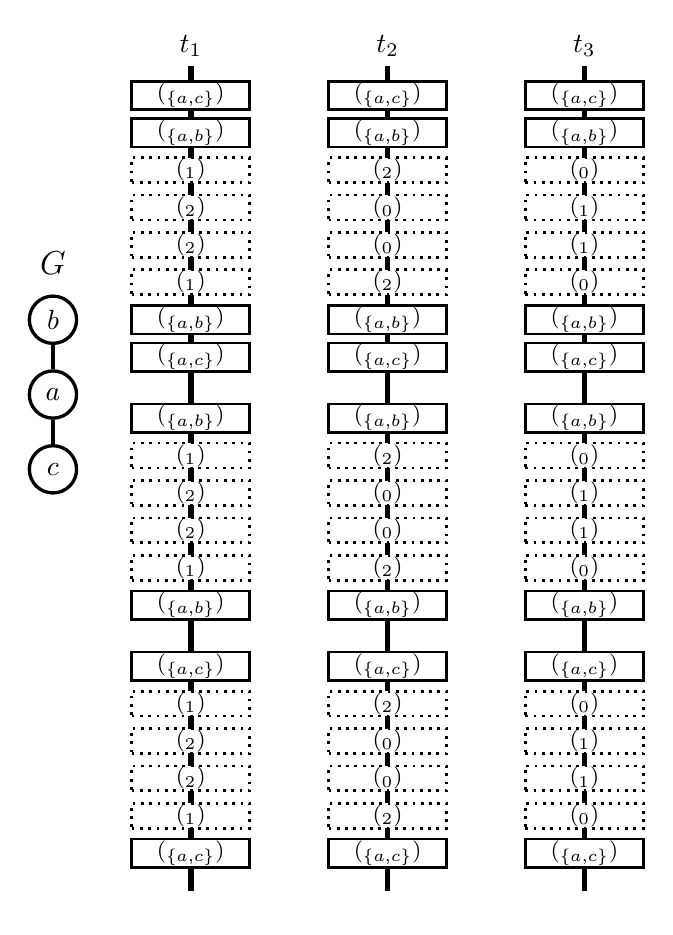
\begin{tikzpicture}[thick,
pre/.style={<-,shorten >= 2pt, shorten <=2pt, very thick},
post/.style={->,shorten >= 3pt, shorten <=3pt,   thick},
seqtrace/.style={line width=2},
und/.style={very thick, draw=gray},
event/.style={rectangle, minimum height=0.8mm, minimum width=15mm,  line width=1pt, inner sep=0.5,},
virt/.style={circle,draw=black!50,fill=black!20, opacity=0}]
\footnotesize


\node[] (G) at (-0.7*\xstep,5.5*\ystep) {\large  $G$};
\node[draw=black, minimum size=6mm, circle, very thick] (1) at (-0.7*\xstep,9*\ystep) {\normalsize $a$};
\node[draw=black, minimum size=6mm, circle, very thick] (2) at (-0.7*\xstep,7*\ystep) {\normalsize $b$};
\node[draw=black, minimum size=6mm, circle, very thick] (3) at (-0.7*\xstep,11*\ystep) {\normalsize $c$};

\draw[-, very thick] (1) to (2);
\draw[-, very thick] (1) to (3);

% \node[] (S11) at (0*\xstep,0.15) {\normalsize $\tr^{(1)}$};
\node[] (S11) at (0*\xstep,0.15) {\normalsize $t_1$};
\node[] (S12) at (0*\xstep,\numevents * \ystep) {};
% \node[] (S21) at (1*\xstep,0.15) {\normalsize $\tr^{(2)}$};
\node[] (S21) at (1*\xstep,0.15) {\normalsize $t_2$};
\node[] (S22) at (1*\xstep,\numevents * \ystep) {};
% \node[] (S31) at (2*\xstep,0.15) {\normalsize $\tr^{(3)}$};
\node[] (S31) at (2*\xstep,0.15) {\normalsize $t_3$};
\node[] (S32) at (2*\xstep,\numevents * \ystep) {};

\draw[seqtrace] (S11) to (S12);
\draw[seqtrace] (S21) to (S22);
\draw[seqtrace] (S31) to (S32);


\node[event, draw=black, fill=white] (11) at (0*\xstep, 1*\ystep + 0*\ybias) {$\acq(\lk_{\{a,c\}})$};
\node[event, draw=black, fill=white] (12) at (0*\xstep, 2*\ystep + 0*\ybias) {$\acq(\lk_{\{a,b\}})$};
\node[event, draw=black, fill=white, dotted] (13) at (0*\xstep, 3*\ystep + 0*\ybias) {$\acq(\lk_1)$};
\node[event, draw=black, fill=white, dotted] (14) at (0*\xstep, 4*\ystep + 0*\ybias) {$\acq(\lk_2)$};
\node[event, draw=black, fill=white, dotted] (15) at (0*\xstep, 5*\ystep + 0*\ybias) {$\rel(\lk_2)$};
\node[event, draw=black, fill=white, dotted] (16) at (0*\xstep, 6*\ystep + 0*\ybias) {$\rel(\lk_1)$};
\node[event, draw=black, fill=white] (17) at (0*\xstep, 7*\ystep + 0*\ybias) {$\rel(\lk_{\{a,b\}})$};
\node[event, draw=black, fill=white] (18) at (0*\xstep, 8*\ystep + 0*\ybias) {$\rel(\lk_{\{a,c\}})$};

\node[event, draw=black, fill=white] (19) at (0*\xstep, 9*\ystep + 1*\ybias) {$\acq(\lk_{\{a,b\}})$};
\node[event, draw=black, fill=white, dotted] (110) at (0*\xstep, 10*\ystep + 1*\ybias) {$\acq(\lk_1)$};
\node[event, draw=black, fill=white, dotted] (111) at (0*\xstep, 11*\ystep + 1*\ybias) {$\acq(\lk_2)$};
\node[event, draw=black, fill=white, dotted] (112) at (0*\xstep, 12*\ystep + 1*\ybias) {$\rel(\lk_2)$};
\node[event, draw=black, fill=white, dotted] (113) at (0*\xstep, 13*\ystep + 1*\ybias) {$\rel(\lk_1)$};
\node[event, draw=black, fill=white] (114) at (0*\xstep, 14*\ystep + 1*\ybias) {$\rel(\lk_{\{a,b\}})$};

\node[event, draw=black, fill=white] (115) at (0*\xstep, 15*\ystep + 2*\ybias) {$\acq(\lk_{\{a,c\}})$};
\node[event, draw=black, fill=white, dotted] (116) at (0*\xstep, 16*\ystep + 2*\ybias) {$\acq(\lk_1)$};
\node[event, draw=black, fill=white, dotted] (117) at (0*\xstep, 17*\ystep + 2*\ybias) {$\acq(\lk_2)$};
\node[event, draw=black, fill=white, dotted] (118) at (0*\xstep, 18*\ystep + 2*\ybias) {$\rel(\lk_2)$};
\node[event, draw=black, fill=white, dotted] (119) at (0*\xstep, 19*\ystep + 2*\ybias) {$\rel(\lk_1)$};
\node[event, draw=black, fill=white] (120) at (0*\xstep, 20*\ystep + 2*\ybias) {$\rel(\lk_{\{a,c\}})$};

%%%%%%%%%%%%%%%%

\node[event, draw=black, fill=white] (21) at (1*\xstep, 1*\ystep + 0*\ybias) {$\acq(\lk_{\{a,c\}})$};
\node[event, draw=black, fill=white] (22) at (1*\xstep, 2*\ystep + 0*\ybias) {$\acq(\lk_{\{a,b\}})$};
\node[event, draw=black, fill=white, dotted] (23) at (1*\xstep, 3*\ystep + 0*\ybias) {$\acq(\lk_2)$};
\node[event, draw=black, fill=white, dotted] (24) at (1*\xstep, 4*\ystep + 0*\ybias) {$\acq(\lk_0)$};
\node[event, draw=black, fill=white, dotted] (25) at (1*\xstep, 5*\ystep + 0*\ybias) {$\rel(\lk_0)$};
\node[event, draw=black, fill=white, dotted] (26) at (1*\xstep, 6*\ystep + 0*\ybias) {$\rel(\lk_2)$};
\node[event, draw=black, fill=white] (27) at (1*\xstep, 7*\ystep + 0*\ybias) {$\rel(\lk_{\{a,b\}})$};
\node[event, draw=black, fill=white] (28) at (1*\xstep, 8*\ystep + 0*\ybias) {$\rel(\lk_{\{a,c\}})$};

\node[event, draw=black, fill=white] (29) at (1*\xstep, 9*\ystep + 1*\ybias) {$\acq(\lk_{\{a,b\}})$};
\node[event, draw=black, fill=white, dotted] (210) at (1*\xstep, 10*\ystep + 1*\ybias) {$\acq(\lk_2)$};
\node[event, draw=black, fill=white, dotted] (211) at (1*\xstep, 11*\ystep + 1*\ybias) {$\acq(\lk_0)$};
\node[event, draw=black, fill=white, dotted] (212) at (1*\xstep, 12*\ystep + 1*\ybias) {$\rel(\lk_0)$};
\node[event, draw=black, fill=white, dotted] (213) at (1*\xstep, 13*\ystep + 1*\ybias) {$\rel(\lk_2)$};
\node[event, draw=black, fill=white] (214) at (1*\xstep, 14*\ystep + 1*\ybias) {$\rel(\lk_{\{a,b\}})$};

\node[event, draw=black, fill=white] (215) at (1*\xstep, 15*\ystep + 2*\ybias) {$\acq(\lk_{\{a,c\}})$};
\node[event, draw=black, fill=white, dotted] (216) at (1*\xstep, 16*\ystep + 2*\ybias) {$\acq(\lk_2)$};
\node[event, draw=black, fill=white, dotted] (217) at (1*\xstep, 17*\ystep + 2*\ybias) {$\acq(\lk_0)$};
\node[event, draw=black, fill=white, dotted] (218) at (1*\xstep, 18*\ystep + 2*\ybias) {$\rel(\lk_0)$};
\node[event, draw=black, fill=white, dotted] (219) at (1*\xstep, 19*\ystep + 2*\ybias) {$\rel(\lk_2)$};
\node[event, draw=black, fill=white] (220) at (1*\xstep, 20*\ystep + 2*\ybias) {$\rel(\lk_{\{a,c\}})$};

%%%%%%%%%%%%%%%%


\node[event, draw=black, fill=white] (21) at (2*\xstep, 1*\ystep + 0*\ybias) {$\acq(\lk_{\{a,c\}})$};
\node[event, draw=black, fill=white] (22) at (2*\xstep, 2*\ystep + 0*\ybias) {$\acq(\lk_{\{a,b\}})$};
\node[event, draw=black, fill=white, dotted] (33) at (2*\xstep, 3*\ystep + 0*\ybias) {$\acq(\lk_0)$};
\node[event, draw=black, fill=white, dotted] (34) at (2*\xstep, 4*\ystep + 0*\ybias) {$\acq(\lk_1)$};
\node[event, draw=black, fill=white, dotted] (35) at (2*\xstep, 5*\ystep + 0*\ybias) {$\rel(\lk_1)$};
\node[event, draw=black, fill=white, dotted] (36) at (2*\xstep, 6*\ystep + 0*\ybias) {$\rel(\lk_0)$};
\node[event, draw=black, fill=white] (37) at (2*\xstep, 7*\ystep + 0*\ybias) {$\rel(\lk_{\{a,b\}})$};
\node[event, draw=black, fill=white] (38) at (2*\xstep, 8*\ystep + 0*\ybias) {$\rel(\lk_{\{a,c\}})$};

\node[event, draw=black, fill=white] (39) at (2*\xstep, 9*\ystep + 1*\ybias) {$\acq(\lk_{\{a,b\}})$};
\node[event, draw=black, fill=white, dotted] (310) at (2*\xstep, 10*\ystep + 1*\ybias) {$\acq(\lk_0)$};
\node[event, draw=black, fill=white, dotted] (311) at (2*\xstep, 11*\ystep + 1*\ybias) {$\acq(\lk_1)$};
\node[event, draw=black, fill=white, dotted] (312) at (2*\xstep, 12*\ystep + 1*\ybias) {$\rel(\lk_1)$};
\node[event, draw=black, fill=white, dotted] (313) at (2*\xstep, 13*\ystep + 1*\ybias) {$\rel(\lk_0)$};
\node[event, draw=black, fill=white] (314) at (2*\xstep, 14*\ystep + 1*\ybias) {$\rel(\lk_{\{a,b\}})$};

\node[event, draw=black, fill=white] (315) at (2*\xstep, 15*\ystep + 2*\ybias) {$\acq(\lk_{\{a,c\}})$};
\node[event, draw=black, fill=white, dotted] (316) at (2*\xstep, 16*\ystep + 2*\ybias) {$\acq(\lk_0)$};
\node[event, draw=black, fill=white, dotted] (317) at (2*\xstep, 17*\ystep + 2*\ybias) {$\acq(\lk_1)$};
\node[event, draw=black, fill=white, dotted] (318) at (2*\xstep, 18*\ystep + 2*\ybias) {$\rel(\lk_1)$};
\node[event, draw=black, fill=white, dotted] (319) at (2*\xstep, 19*\ystep + 2*\ybias) {$\rel(\lk_0)$};
\node[event, draw=black, fill=white] (320) at (2*\xstep, 20*\ystep + 2*\ybias) {$\rel(\lk_{\{a,c\}})$};

%%%%%%%%%%%%%%%%
\end{tikzpicture}
}
\caption{
Reduction for $\W{1}$-hardness proof. Graph $G$ has $n = 3$ nodes and $2$ edges.
Parameter $c = 3$.
\Andreas{These figures are too big. Maybe introduce (graphically) the notation $\acq(\lk_1,\lk_2)$ to denote nested locking, then using in this and next figure.}
}
\figlabel{w1-hardness}
\end{figure}